\documentclass[11pt]{article}
\usepackage{graphicx}
\usepackage{setspace}
\usepackage{hanging}
\pagestyle{headings}
\linespread{1.6}
\raggedright
\parindent=15pt
\begin{document}
\title{Hack All The History! \\ Hackers 1959 - 1991}
\author{Kevin Vilbig}
\maketitle
\thispagestyle{empty}
\begin{center}
An undergraduate honors thesis submitted in partial fulfillment of the \\
requirements for a degree of \\
Bachelor of Science\\
in\\
University Honors \\
and \\
Social Science\\
Richard Beyler\\
Portland State University\\
2013 \\
This document was prepared with \LaTeX.\\
This work is licensed under the Creative Commons Attribution-ShareAlike 3.0 Unported License. To view a copy of this license,\\ visit http://creativecommons.org/licenses/by-sa/3.0/.
\end{center}

\newpage
\pagenumbering{roman}
Thanks to Richard Beyler for advising me on this project. Also, thanks to Ann Marie Fallon, Lawrence Wheeler, Kathleen Merrow, Charles Baumbach, Mary Domski, Debora Stott and Lee Shaker for introducing me to the research skills and ideas that I needed to complete this project. There are many others who have helped me develop as a writer and a scholar over the years as well, but these are the principal ones.

\newpage

\begin{figure}
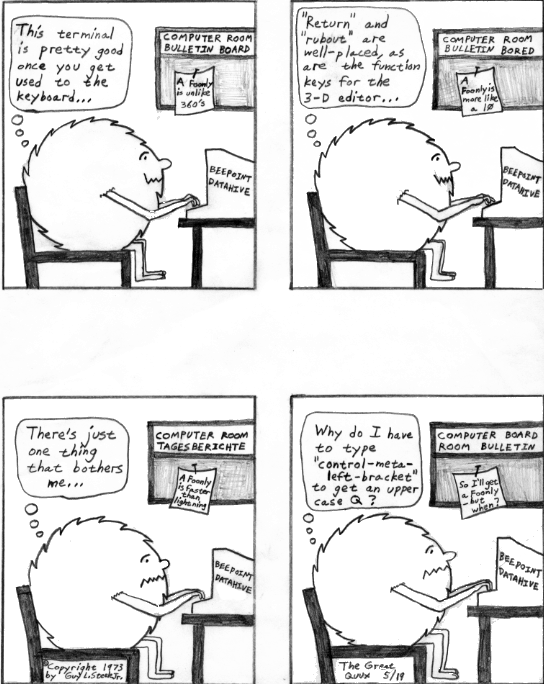
\includegraphics[width=4.5in]{73-05-19.png}
\caption{Crunchly cartoon from the Jargon File}
\end{figure}

\newpage

\tableofcontents

\newpage
\pagenumbering{arabic}
\setcounter{page}{1}
\section{Introduction}

\subsection{What is a hacker?}
\begin{quote}
hacker: n.
    [originally, someone who makes furniture with an axe] \\
    1. A person who enjoys exploring the details of programmable systems and how to stretch their capabilities, as opposed to most users, who prefer to learn only the minimum necessary. RFC1392, the Internet Users' Glossary, usefully amplifies this as: A person who delights in having an intimate understanding of the internal workings of a system, computers and computer networks in particular.\\
    2. One who programs enthusiastically (even obsessively) or who enjoys programming rather than just theorizing about programming. \\
    3. A person capable of appreciating hack value. \\
    4. A person who is good at programming quickly. \\
    5. An expert at a particular program, or one who frequently does work using it or on it; as in ‘a Unix hacker’. (Definitions 1 through 5 are correlated, and people who fit them congregate.) \\
    6. An expert or enthusiast of any kind. One might be an astronomy hacker, for example. \\
    7. One who enjoys the intellectual challenge of creatively overcoming or circumventing limitations. \\
    8. [deprecated] A malicious meddler who tries to discover sensitive information by poking around. Hence password hacker, network hacker. The correct term for this sense is cracker.
    \footnote{Eric S. Raymond, \emph{The Jargon File version 4.4.7} (2003), http://www.catb.org/jargon/html/H/hacker.html.}

\end{quote}

Within the incubator of an MIT edifice, building 26, a new subculture was created by the advanced defense research wing of the Department of Defense, DARPA.
\footnote{Katy Kline, "A Brief Architectural History of MIT" in \emph{Art and Architecture at MIT: A Walking Tour of the Campus} (Cambridge: MIT Press, 1988)}
The philosophy of this culture reflected much of the popular youthful idealism of the day with a techno-Utopian bent. This institutional microcosm of the American cultural landscape nurtured the development of hackers as a cultural phenomenon.
\footnote{Douglas Thomas, \emph{Hacker Culture} (Minneapolis: University of Minnesota 2002).}
The world  was hours away from nuclear apocalypse. All schoolchildren were taught about the frightful power of the nuclear bomb from a young age, and even the most stubbornly optimistic must have realized, deep down, that the only result of nuclear engagement was going to be nothing less than massive, Earthshaking annihilation.
\footnote{United States Congress, "The Effects of Nuclear War" by Lionel S. Johns, et al., (Washington, D.C.:GPO, 1979), http://ota.fas.org/reports/7906.pdf.}

How does someone become a hacker?
\footnote{Eric S. Raymond, "How To Become A Hacker" (20 May 2012), http://www.catb.org/esr/faqs/hacker-howto.html.}
A better question might be, where do the hackers fit into these greater institutional systems? As often as not, those taking the name hacker are dropouts and troublemakers as far as institutions were concerned. They're often seen as deviants or as with the recent tragedy of Aaron Swartz's suicide, criminals looking to spend a considerable time in prison. With these risks, many of the people who identify as hackers don't publicly share their techniques and stories. The name has been demonized and deified by popular culture. Is it that the evidence of the spread of hacker culture has been lost in the wires, even with only a fifty-five year history?

Hackers, as a codified culture based upon these artifacts, have a simple test on whether someone is a hacker or not. It depends on the definition of hacker, normal people tend to see the 8th definition as the sole definition. Some who assume the identity of hacker themselves take a much wider view.  Richard Stallman, the motive force behind the free software movement and author of the GNU Public License defines it as, 

\begin{quote}
It is hard to write a simple definition of something as varied as hacking, but I think what these activities have in common is playfulness, cleverness, and exploration. Thus, hacking means exploring the limits of what is possible, in a spirit of playful cleverness. Activities that display playful cleverness have "hack value".
\footnote{Richard Stallman, "On Hacking" (2002), http://stallman.org/articles/on-hacking.html.}
\end{quote}

Stallman hopes to divorce his definition of hacker from the computational security focus in the popular definition, but for these purposes we cannot completely hack away the strings of history and let language fly free. The influence between the underground groups who may have stolen the word and the institutional culture of hackers runs deep, because the congruence between these groups, if not necessarily in individual people. The overlap can be found in many of their ideals, means, and motivations. This doesn't tell the whole story. We have to be a bit more specific about origins to successfully differentiate the real hackers from the charlatans and script kiddies.
\footnote{Script kiddies is a hacker term for someone who manages to learn how to use premade software tools to cause mayhem without understanding or even intending to learn about the principles that make them work.}

The definition that we are running with pins hackers as a distinct cultural phenomenon that began in the US universities, primarily MIT. These hackers had a common interest in programming the interactive computer systems that were available to students, faculty, and some notable visitors. They developed and codified their jargon and values while creating much of the basis for how we use computers to this day. Their cultural values then spread, some via the ARPANET, some via various communities surrounding electronic bulletin board systems and some via the hackers themselves moving to new institutions. Hackers are the people who get a thrill out of interactive computing. They enjoy computing for its own sake, maybe in a world out of control, it gave them the ability to at least control a small slice of reality. 1959 - 1991 are the years we're naming as key to the creation of the computer hackers as a discrete cultural group. 1959 is the first encounter of Peter Samson with the TX-0 in the second floor of MIT's Building 26. 1991 is the year when then grad student Linus Torvalds released the first public release of his now ubiquitous operating system kernel, named Linux. We're ending the narrative there to avoid discussing any effects of that, as volumes have already been written.

\subsection{Hacker Ethic}

\begin{quote}
The hacker ethic is shorthand for a list of tenets, and it includes a mix of aesthetic and pragmatic imperatives: a commitment to information freedom, a mistrust of authority, a heightened dedication to meritocracy, and the firm belief that computers can be the basis for beauty and a better world.\footnote{Gabriela Coleman, \emph{Coding Freedom} (Princeton: Princeton University Press, 2013), 17.}
\end{quote}

The popular concept of hackers paints hackers as lone genius types, but the hacker ethic was a product of an institutional environment. This is key, because the ten tenets of the ethic are still displayed online, with only a minor addendum, almost thirty years later, by one of the self-identifying hacker groups out of Berlin, the Chaos Computer Congress, or CCC.
\footnote{Chaos Computer Congress. "Hackerethik," (Berlin 2013), http://ccc.de/de/hackerethik.} This suggests a continuity of ideal motivation that is core to the discussion. Though, it is doubtful that these ideals hold tractably outside of the institutional environments in which they were born. The goal of this paper is to explore one idea that has recieved a lot of recent attention: Information should be free. The goal is to to ask the question: Should information be free? Within a university or other research institution, or when the information has little to no commercial, strategic, political, or popular value, the answer is why not? There was no reason to even think about software licensing when the software was written for a Digital Equipment Corporation machine, like the PDP-1, that had less than a hundred installations.
\footnote{Digital Equipment Corporation, \emph{Digital Equipment Corporation: Nineteen Fifty-Seven to the Present} (DEC Press, 1978), pg. 3}
Within those boundaries and constraints, information sharing was more beneficial than harmful. As computing spread throughout the rest of the world, this becomes a much trickier proposition. Information is created by people and does not have some intrinsic property of freedom. This ideal created a problematic juxtaposition between a technical countercultural elite and normal society.

\newpage
\section{Common Evidence,  Divergent Methodology}

There have been scholars from all over the spectrum of academia turning their attention toward the odd phenomenon of Hackerdom. One has to realize that any mention of open source or free software is necessarily related to hackers. We have anthropologists,
\footnote{Chris Kelty, \emph{Two Bits : The Cultural Significance of Free Software} (Durham: Duke University Press 2008), and Coleman, \emph{Coding Freedom.}}
business, marketing, political science, criminal justice,
\footnote{Thomas J. Holt, "Subcultural Evolution? Examining the Influence of On and Off-line Experiences on Deviant Subcultures. Deviant Behavior 28:2, 171-198 and Steve Schroeder, \emph{The Lure the True Story of How the Department of Justice Brought Down Two of the World's Most Dangerous Cyber Criminals.} (Boston: Course Technology PTR. 2012) http://site.ebrary.com/id/10448180 and Donn B. Parker, \emph{Fighting Computer Crime,} (New York: Scribner, 1983)}
philosophers,
\footnote{Pekka Himanen, \emph{The Hacker Ethic, and the Spirit of the Information Age}, (New York: Random House, 2001)}
 and others.
\footnote{McKenzie Wark, \emph{A Hacker Manifesto.} (Cambridge, MA : Harvard University Press, 2004).} 
This isn't an exhaustive list, as there are some tens of thousands of articles and books available with a database search and it would be overkill to survey them all.

The common texts that are often cited include Levy's \emph{Hackers: Heroes of the Computer Revolution}. Levy's text truly is a seminal work that defines hackers' origins, pinning them to a certian historical time and place. Many of the scholars also give a cite or two to Richard Stallman's essays on Free Software. They also turn to Eric S. Raymond's \emph{Cathedral and the Bazaar.} as another primary text, written by hackers, for hackers. It covers the phenomenon that occurred after the birth of the free and open source microcomputer operating system.  Raymond is also known for publishing the \emph{Jargon File} as \emph{The New Hacker's Dictionary}. This tome is full of humor about dealing with the complexity and esoteric nature of the networked computer systems of the day.
\footnote{Eric S. Raymond, \emph{The New Hacker's Dictionary - 3rd edition} (Cambridge: The MIT Press 1996).}
A single computer is already an extremely complex electronic machine, and when more and more of them are connected together the complexity compounds.

These digital artifacts were transmitted as the ARPANET connected more institutions and hackers tutored new members in the way of the hack. It is important to survey the sources published by the emergent members of the digital underground, known by their handles such as Knight Lightning and Emmanuel Goldstein, of \emph{Phrack} and \emph{2600}. There is also a massive archive of material curated by Jason Stott, a non-academic hacker-historian who runs the community archive, Textfiles.com. The technical articles aren't terribly useful for this project as they don't say anything about the social and political motivations of hackers. We are looking for things that suggest the philosophical and political motivations of the publishers rather than something like assembler code for a Commodore 64 BASIC interpreter.

The text that defines this culture to most academics is Stephen Levy's \emph{Hackers: Heroes of the Computer Revolution}  His work makes for a great mythological back story, and seemed to also have an amplification effect on the adoption of hacker values throughout the rest of society.  So, if hackers, and the whole concept of a hack as anything but something to do with axes started as an institutional in-joke for MIT students.
\footnote{IHTFP FAQ,  http://hacks.mit.edu/Hacks/misc/faq.html, accessed Feb 2013}
How did this name pass from within those boundaries to the rest of the world? 1984 was a big year for the open expression of hacker culture, as it also saw the inception of the two public hacker 'zines, \emph{2600 Magazine}, commonly available in print, and \emph{Phrack}, an electronic publication. These are not the only publications, but they are probably the most famous and widely circulated.

\newpage
\section{Clay Tablets and Telegraphs}

\begin{figure}[ht!]
\center
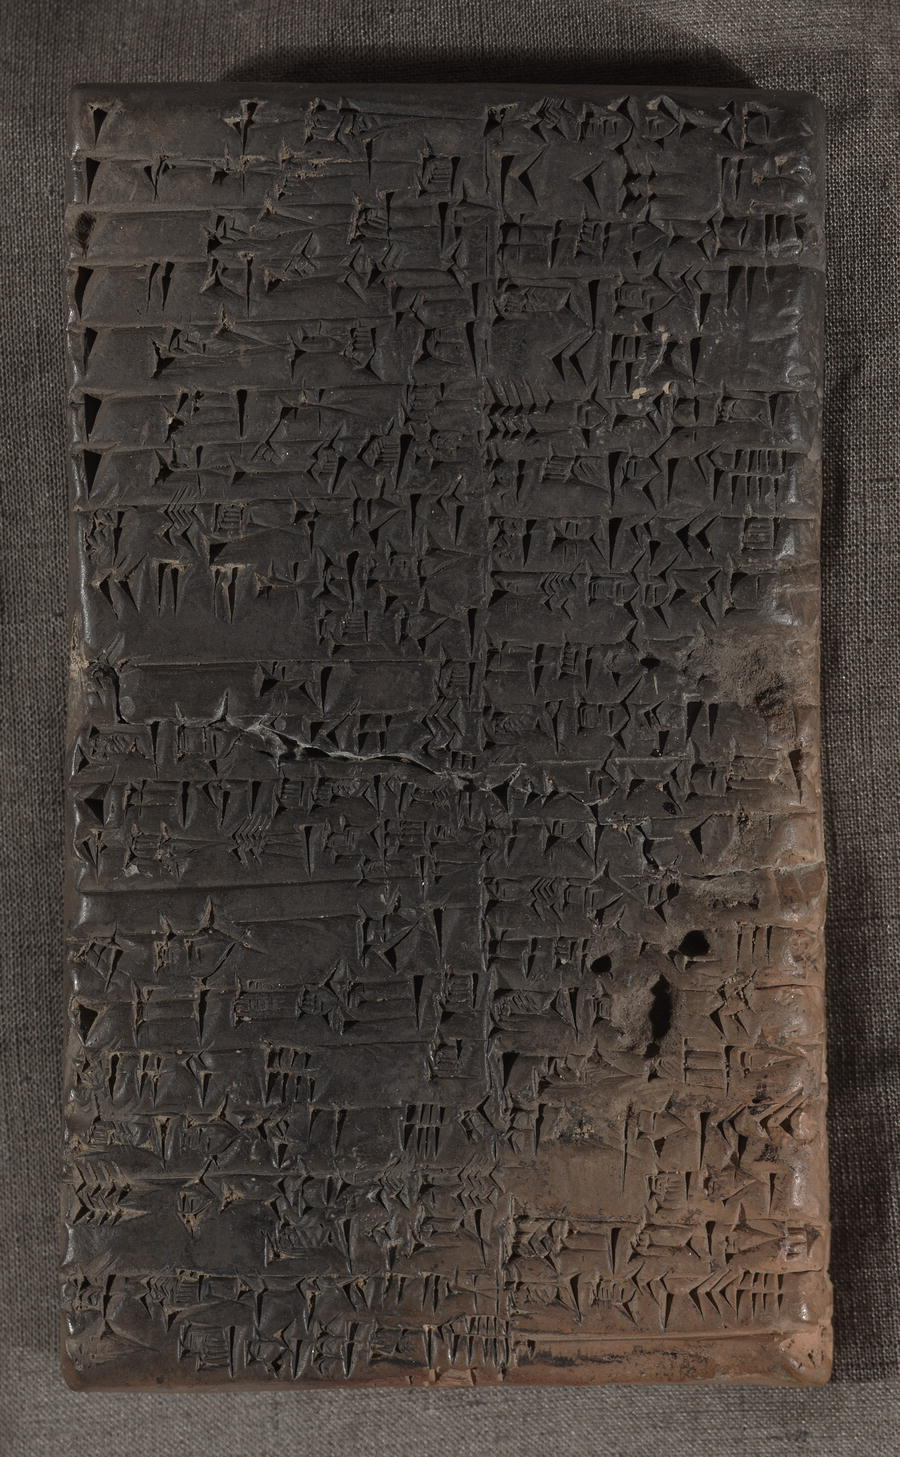
\includegraphics[width=70mm, angle=90]{cuniform_tablet.jpg}
\caption{A cunieform tablet containing ancient payroll information. Amar-Suen. Disbursement of wages. \emph{Cuneiform Tablets: From the Reign of Gudea of Lagash to Shalmanassar III.} Library of Congress, African and Middle Eastern Division, Washington, D.C. 20540. 2039 BCE. http://memory.loc.gov/cgi-bin/query/h?intldl/cunei:@FIELD(DOCID+@BAND(@lit(amcune000013)))}
\end{figure}

A wide array of sociological and technological factors had to come together to create the cybernetic environment that allowed hackers to flourish. The people with the requisite skills and desire to build and populate it had to be in the right places at the right times: in front of the terminal's otherworldly glow. The intent here is to draw a historical through-line between the ideal systems, like maps and nomenclatures, and the physical computer systems that people interacted with. Many of the ways with which we interact with information have remained fundamentally unchanged from these ideal structures,  most of which were created during the Enlightenment and Scientific Revolution. We still display graphical data on Cartesian coordinate systems in maps and charts and still store sorted, indexed and cross referenced data as we have in dictionaries and encyclopedias and libraries for hundreds of years.
\footnote{Daniel Headrick, \emph{When Information Came of Age.} (New York : Oxford University Press. 2000).}

\begin{figure}[ht!]
\center
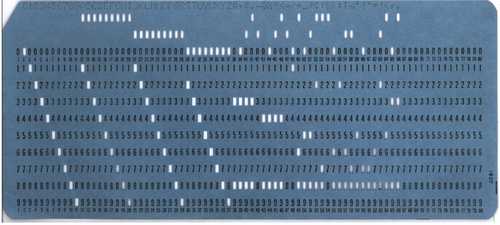
\includegraphics[width=90mm]{500px-Blue-punch-card-front-horiz.png}
\caption{An 80-column punched card of the type most widely used in the 20th century. Card size was 7 3⁄8 in × 3 1⁄4 in (187.325 mm × 82.55 mm). This example displays the 1964 EBCDIC character set, which added more special characters to earlier encodings. Wikimedia foundation. (http://en.wikipedia.org/wiki/Punched\_card) }
\end{figure}

The fundamental systems that were put into place are the actual physical medium that carry signals. Telegraphs, telephones, radios, and televisions all already worked to transmit and receive arbitrary analog signals. Abstractly talking about the system as some monolith doesn't really help to understand the political forces that went along with their construction. The old telegraph systems and new optical fibers even follow the same paths underneath the ocean. The previous century's telegraph systems and the computer data systems of today are very similar, but instead of doing the encryption and decryption via the human telegraph operators, we have automated the translation of the symbols so that they can be transmitted as electrical pulses over wires and displayed as the familiar language without human intervention. Every e-mail you send is translated into a binary encoding and then decoded prior to its display on the other end.

\begin{figure}[ht!]
\center
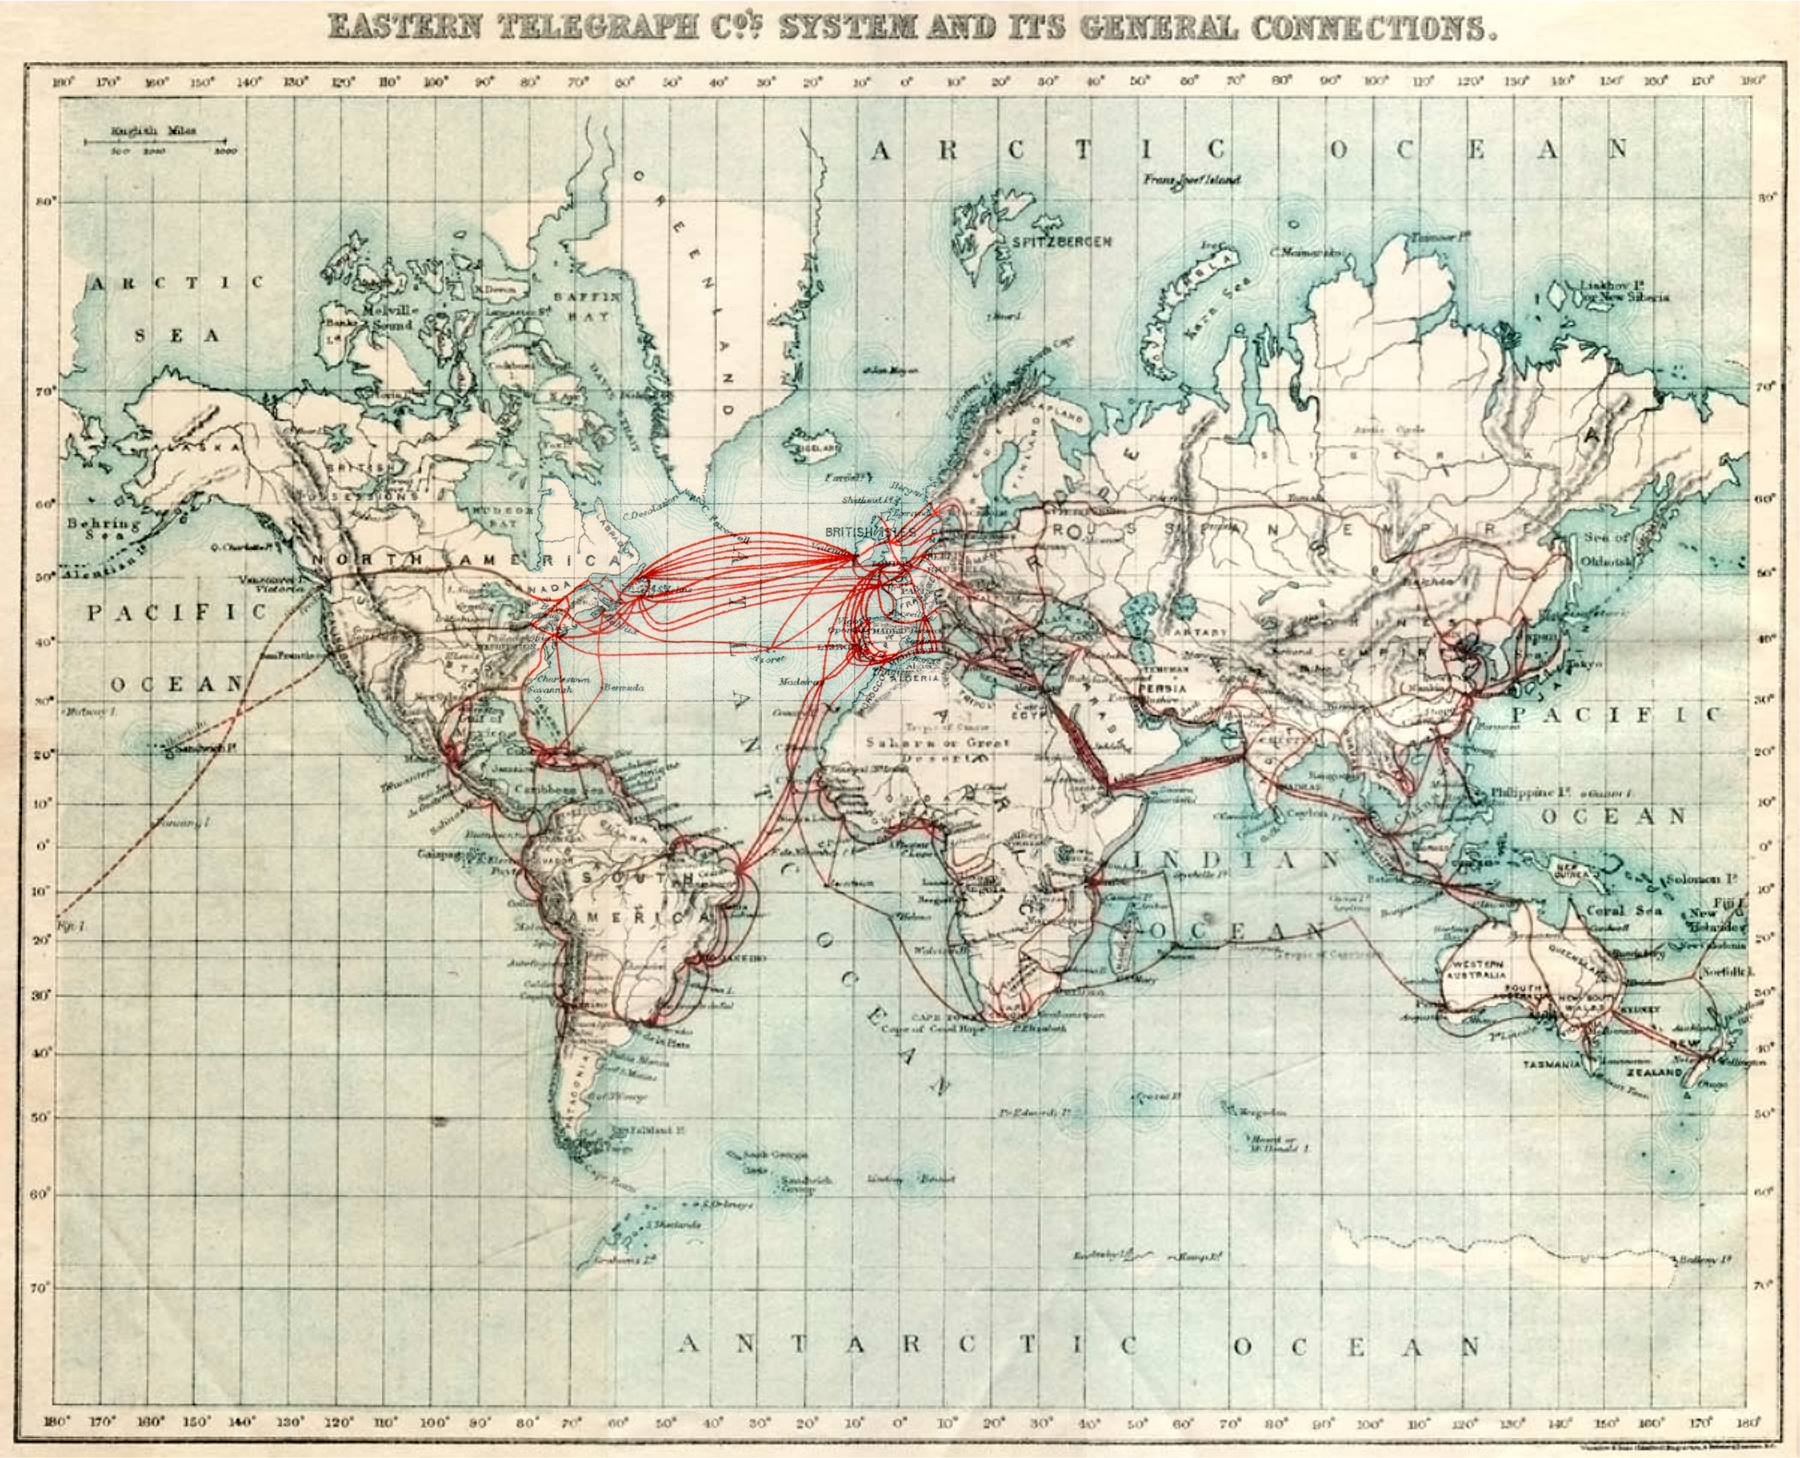
\includegraphics[width=110mm]{1901_Eastern_Telegraph_cables.png}
\caption{Map of Eastern Telegraph's cable network. Wikimedia Foundation. 1901.}
\end{figure}

\begin{figure}[ht!]
\center
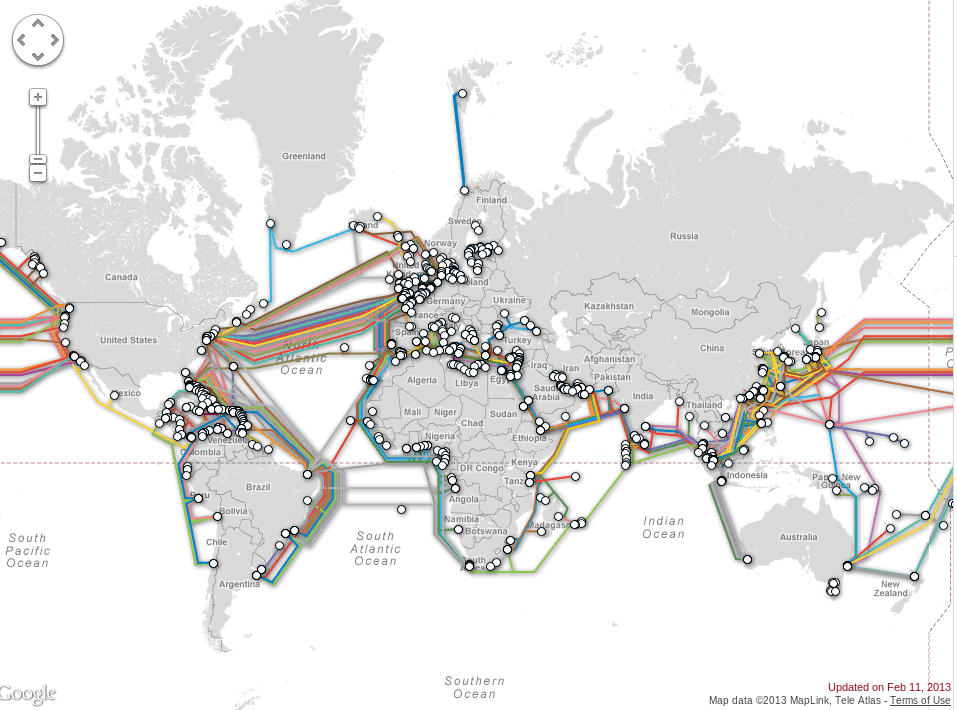
\includegraphics[width=110mm]{sub_cable_map.png}
\caption{Submarine Cable Map. Global Bandwidth Research Service. 2013. Screen Capture of Interactive map. http://www.submarinecablemap.com/}
\end{figure}

Telegraph cables and telephone systems began their life as a command and control network for various military industrial complexes across the world, the fears of the 60s Berkeley protesters who wore punch-cards around their necks have become more realized than they would ever imagine.
\footnote{Daniel Headrick, \emph{The Invisible Weapon} (New York: Oxford University Press, 1991).}\begin{quote}The
“information machine” metaphor
was
made
explicit
in
Hal
Draper’s history
of
the
Free
Speech
Movement.
Draper,
a
participant
in
the
movement, wrote
that the student
in
the
“mass
university
of
today’’
feels
that
it
is
“an
overpow-
ering,
over-towering,
impersonal, alien machine
in
which he is
nothing
but
a cog
going through
pre-
programmed
motions-the
‘IBM’
syndrome”
(153).*
Punch
cards
were
the
symbol
of
information
machines,
and
so
they became
the
symbolic
point
of
attack.
Todd Gitlin
sums
up-and dismisses-
the
Free
Speech Movement as
a protest against
“suburban
blandness, middle-class
impersonality,
and
folding-spindling-and-mutilating
universities”
(164)
\footnote{Stephen Lubar, ""Do Not Fold, Spindle or Mutilate": A Cultural History of the Punch Card," \emph{Journal of American Culture} 15, no. 4 (1992): 46.}
\end{quote}
The world of today, where our names, faces, and histories are run through computers every day for everything from facial recognition, employment verification, credit, and financial transactions. It's probably no accident that 1984 was the year that these hacker 'zines began their aboveground publication. These military-industrial-complex roots are a key to the problematic nature of this whole hacker phenomenon. This cannot be overstated.

The survival of this military command and control, with the pressures of the Cold War strategic thinking, required the expansion and creation of a new kind of communications network that was decentralized, robust, and fault-tolerant. The packet-switched network was able to relay messages regardless of the state of the network.
\footnote{Janet Abbate, \emph{Inventing the Internet} (Cambridge: MIT Press, 1999).}
This means that even if a part of the network was destroyed or even just glutted with traffic, the design of the system automatically rerouted the flow of information. Intercontinental ballistic missiles carrying nuclear powered payloads gave nations the ability to project massively lethal force at any point on the planet at short notice.

The story of hacker culture is intertwined with some key advances in computer and telecommunication technology. The institutional computer networking systems allowed this nascent culture to spread it's roots through the networks arterially and the microcomputer allowed hobby users to connect together in local communities. We should follow the line of reasoning that Headrick communicates as the notion that networked computer systems another step along a centuries old track.
\footnote{Daniel Headrick, \emph{When Information Came of Age} ( 217.}
Humans have been using encoded networks to transmit information for millennium, whether via smoke signals or electric pulses along wires, the results are similar.

\newpage
\section{Institutional Revolutionaries}

The first part of hacker history is the gestation of the culture within MIT and its ensuing spread to Stanford and other universities during the 1960s.\footnote{Levy, pg 138} There isn't much to say here that hasn't already been exhaustively documented, discussed, and distributed. The basic story is that the global culture of hacking started in a specific place at a specific time. Peter Samson is the grandfather of hacking as we see today. His explorations into the steam tunnels at MIT, finding the unlocked room with the TX-0 computer, pictured in Fig 6. He and his buddies, under the supervision of John McCarthy, pioneered computer technology, developing the first applications for computer generated music, computer games, as well as assembler programs that allowed for interactive computer programming.

\begin{figure}[ht!]
\center
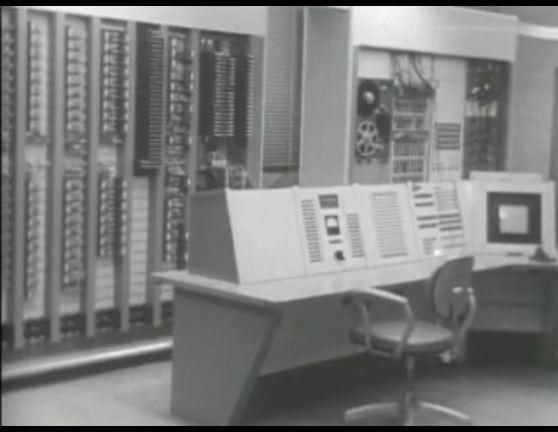
\includegraphics[width=80mm]{TX-0.jpg}
\caption{The TX-0: screenshot from MIT CSAIL video Archive http://www.csail.mit.edu/videoarchive/history/aifilms/museum-105}
\end{figure}

This began a culture of computing where hacking into the late hours of the morning was necessary, because the more normal working hours were filled up with graduate students or professors working on their projects. The original generation of hackers were making sure that the computing resources available were used constantly. So they would end up hanging out by the machine, waiting, just in case one of the scheduled users failed to show. This practice created a culture of hanging around the machine while also fueling their obsession. Hackers have a relatively long history as academic targets of scorn. Joseph Weizenbaum was a professor at MIT during the beginning, when the Tech Model Railroad Club hackers coined the term and codified much of the jargon that is still in use today. He dedicated a chapter of his 1976 text to a diatribe against some of the TMRC hackers, though he does not employ that name. He stops short of calling them smelly weirdos, just.
\footnote{Joseph Weizenbaum, "Science and the compulsive programmer." \emph{Computer Power and Human Reason.} (San Fransisco: W.H. Freeman and Company, 1976).}  

The culture spread outside of this core group quickly as more machines opened up and more people became aware of the practice. The culture spread, codified in common cultural artifacts like the abeforementioned Jargon File. Stanford soon opened their Artificial Intelligence laboratory, acronymed to SAIL. Again, going into the technical details of their projects, while being absolutely fascinating and something that this author has "wasted" an enormous amount of time on over the course of this project, would not advance the argument about the origins and tenability of this ideal of information freedom. The fact that these SAIL hackers were intentionally created and meant to replicate the success of MIT is what is important to take away here. Similar institutional systems for computer users were also instantiated at Berkeley, going by the name Project Genie.
\footnote{Paul Spinrad and Patti Meagher. "Project Genie: Berkeley’s piece of the computer revolution" \emph{Forefront} (Fall 2007) http://coe.berkeley.edu/news-center/publications/forefront/archive/forefront-fall-2007/features/berkeley2019s-piece-of-the-computer-revolution}

\newpage
\section{Homebrew Clubs to Underground, Emergent}

Some of the first computer links were established with machines like this acoustic coupler. (Fig. 7) The first of these devices was developed by Livermore Data Systems in 1963. This box allowed machines to be connected via telephone lines for communication without having a direct electrical link to the system. Anyone who's had a lightning strike take out their telephone knows the possible risks, and when the machines in question cost in the order of hundreds of thousands of dollars, it's a good idea. These simple non-switched links were sufficient for the time, but long distance transmission of the data was prohibitively expensive, considering the speed at which these devices could communicate. These simple links evolved into the development of the ARPANET, packet switching, and the related technologies that underlie the Internet as we experience today. These developments have been extensively documented and there is no reason for us to rehash this story yet another time.
\footnote{Janet Abbate, \emph{Inventing the Internet} (Cambridge: MIT Press, 1999).}

\begin{figure}[ht!]
\center
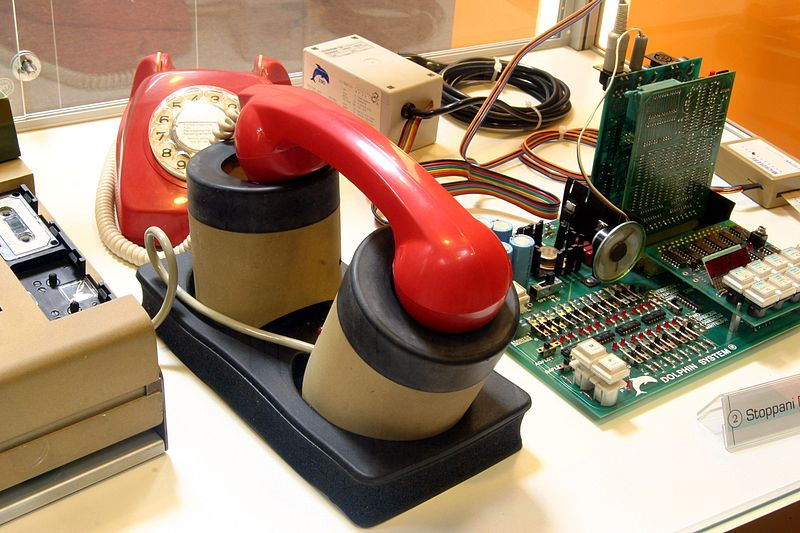
\includegraphics[width=80mm]{800px-Coupleur-accoustique-IMG_0298.JPG}
\caption{Acoustic Coupler via the Wikimedia Foundation http://en.wikipedia.org/wiki/Acoustic\_coupler}
\end{figure}

\subsection{Phreaking}

The difference between having a telephone system that can connect the line, amplify, and transmit the voice calls and a system that can do that while also logging this and properly billing the customer is immense. The logging and billing system is as complex, if not more complex than the telephone network itself. It added an entire layer alongside, intertwined with the telephone calls and telegraph messages, Ma Bell wasn't just concerned with the transmission of the voice signals.It was necessary to transmit control tones and billing information as well.
\footnote{C. Breen, and Dahlbom, C. A. "Signaling Systems for Control of Telephone Switching," \emph{The Bell System Technical Journal} 39:6. Nov 1960.}

John Draper, a.k.a. Captain Crunch, and some of his buddies were playing around with the Bell monopoly's telephone system through the late 60s and early 70s.  The automation of the switching systems in the network gave a small segment of the creative youth, known colloquially as phreaks or phreakers, the ability to dance across the wires. They knew how the phone system worked and used this knowledge to span a circuit three times around the globe to call the pay-phone in the next booth over, but mostly, this knowledge served to give people the ability to place calls that were billed to someone else, or nobody at all.
\footnote{Ron Rosenbaum, "Secrets of the Little Blue Box" \emph{Esquire} 1971.}

It's no secret that Apple founders began their forays into business by selling devices that facilitated this exact practice. They're known as Blue Boxes.
\footnote{
Stephen Wozniak, "Blue Box" http://www.woz.org/category/tags/blue-box, accessed May 21, 2013.
}
These devices were a modified tone dialer that allowed a person to generate the system control tones. This meant they had direct control over the telephone switching machinery. This meant that with device smaller than a paperback book, any person tutored in its use could manipulate the system into giving free calls.

\subsection{Homebrew Computer Club vs. Gates}
\begin{figure}[ht!]
\center
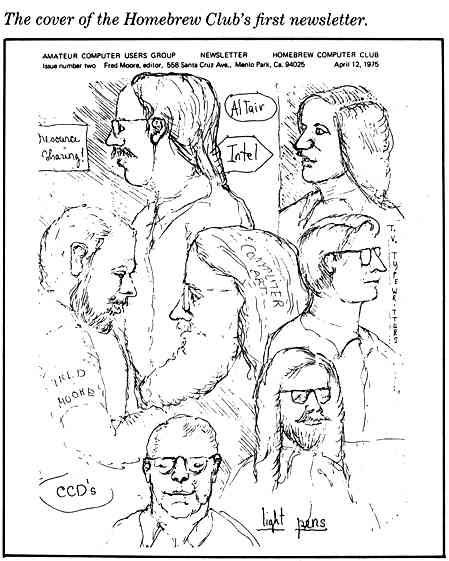
\includegraphics[width=100mm]{homebrew_cover.jpg}
\caption{Stephen Wozniak, "Homebrew and how the Apple came to be," \emph{Atari Archives.} http://www.atariarchives.org/deli/homebrew\textunderscore and\textunderscore how \textunderscore the\textunderscore apple.php }
\end{figure}

\begin{verbatim}
PRINT "HELLO WORLD!"
\end{verbatim}

All new programmers will undoubtedly run into some variation of the preceding  program that allows you to see the basic input and output facilities of your machine. The version you see above is BASIC, one of the first consumer-grade languages and also began the global tradition of pirating Microsoft's software.
\footnote{Adrian Johns, \emph{Piracy: The Intellectual Property Wars from Gutenberg to Gates} (University of Chicago Press, 2010).}
The most poignant evidence of this is Bill Gates' "Open Letter to Hobbyists".
\footnote{Bill Gates, "An Open Letter to Hobbyists," \emph{Various Sources} (1975) http://en.wikipedia.org/wiki/Open\_Letter\_to\_Hobbyists}
Bill Gates wrote his "Open Letter to Hobbyists" decrying the widespread practice of piracy. Microsoft was using a per-copy royalty model for payment with their distributers, so each unauthorized copy hurt his bottom line. This is the first time such an issue was even brought up. It was considered an integral part of hacker culture to openly share the programs that were created, and this is one of the first examples of software piracy, and definitely one of the most famous early examples of conflict between the proprietary and free software ways and generally illustrates the issues with development and distribution of commercial software that continues today.

\begin{figure}
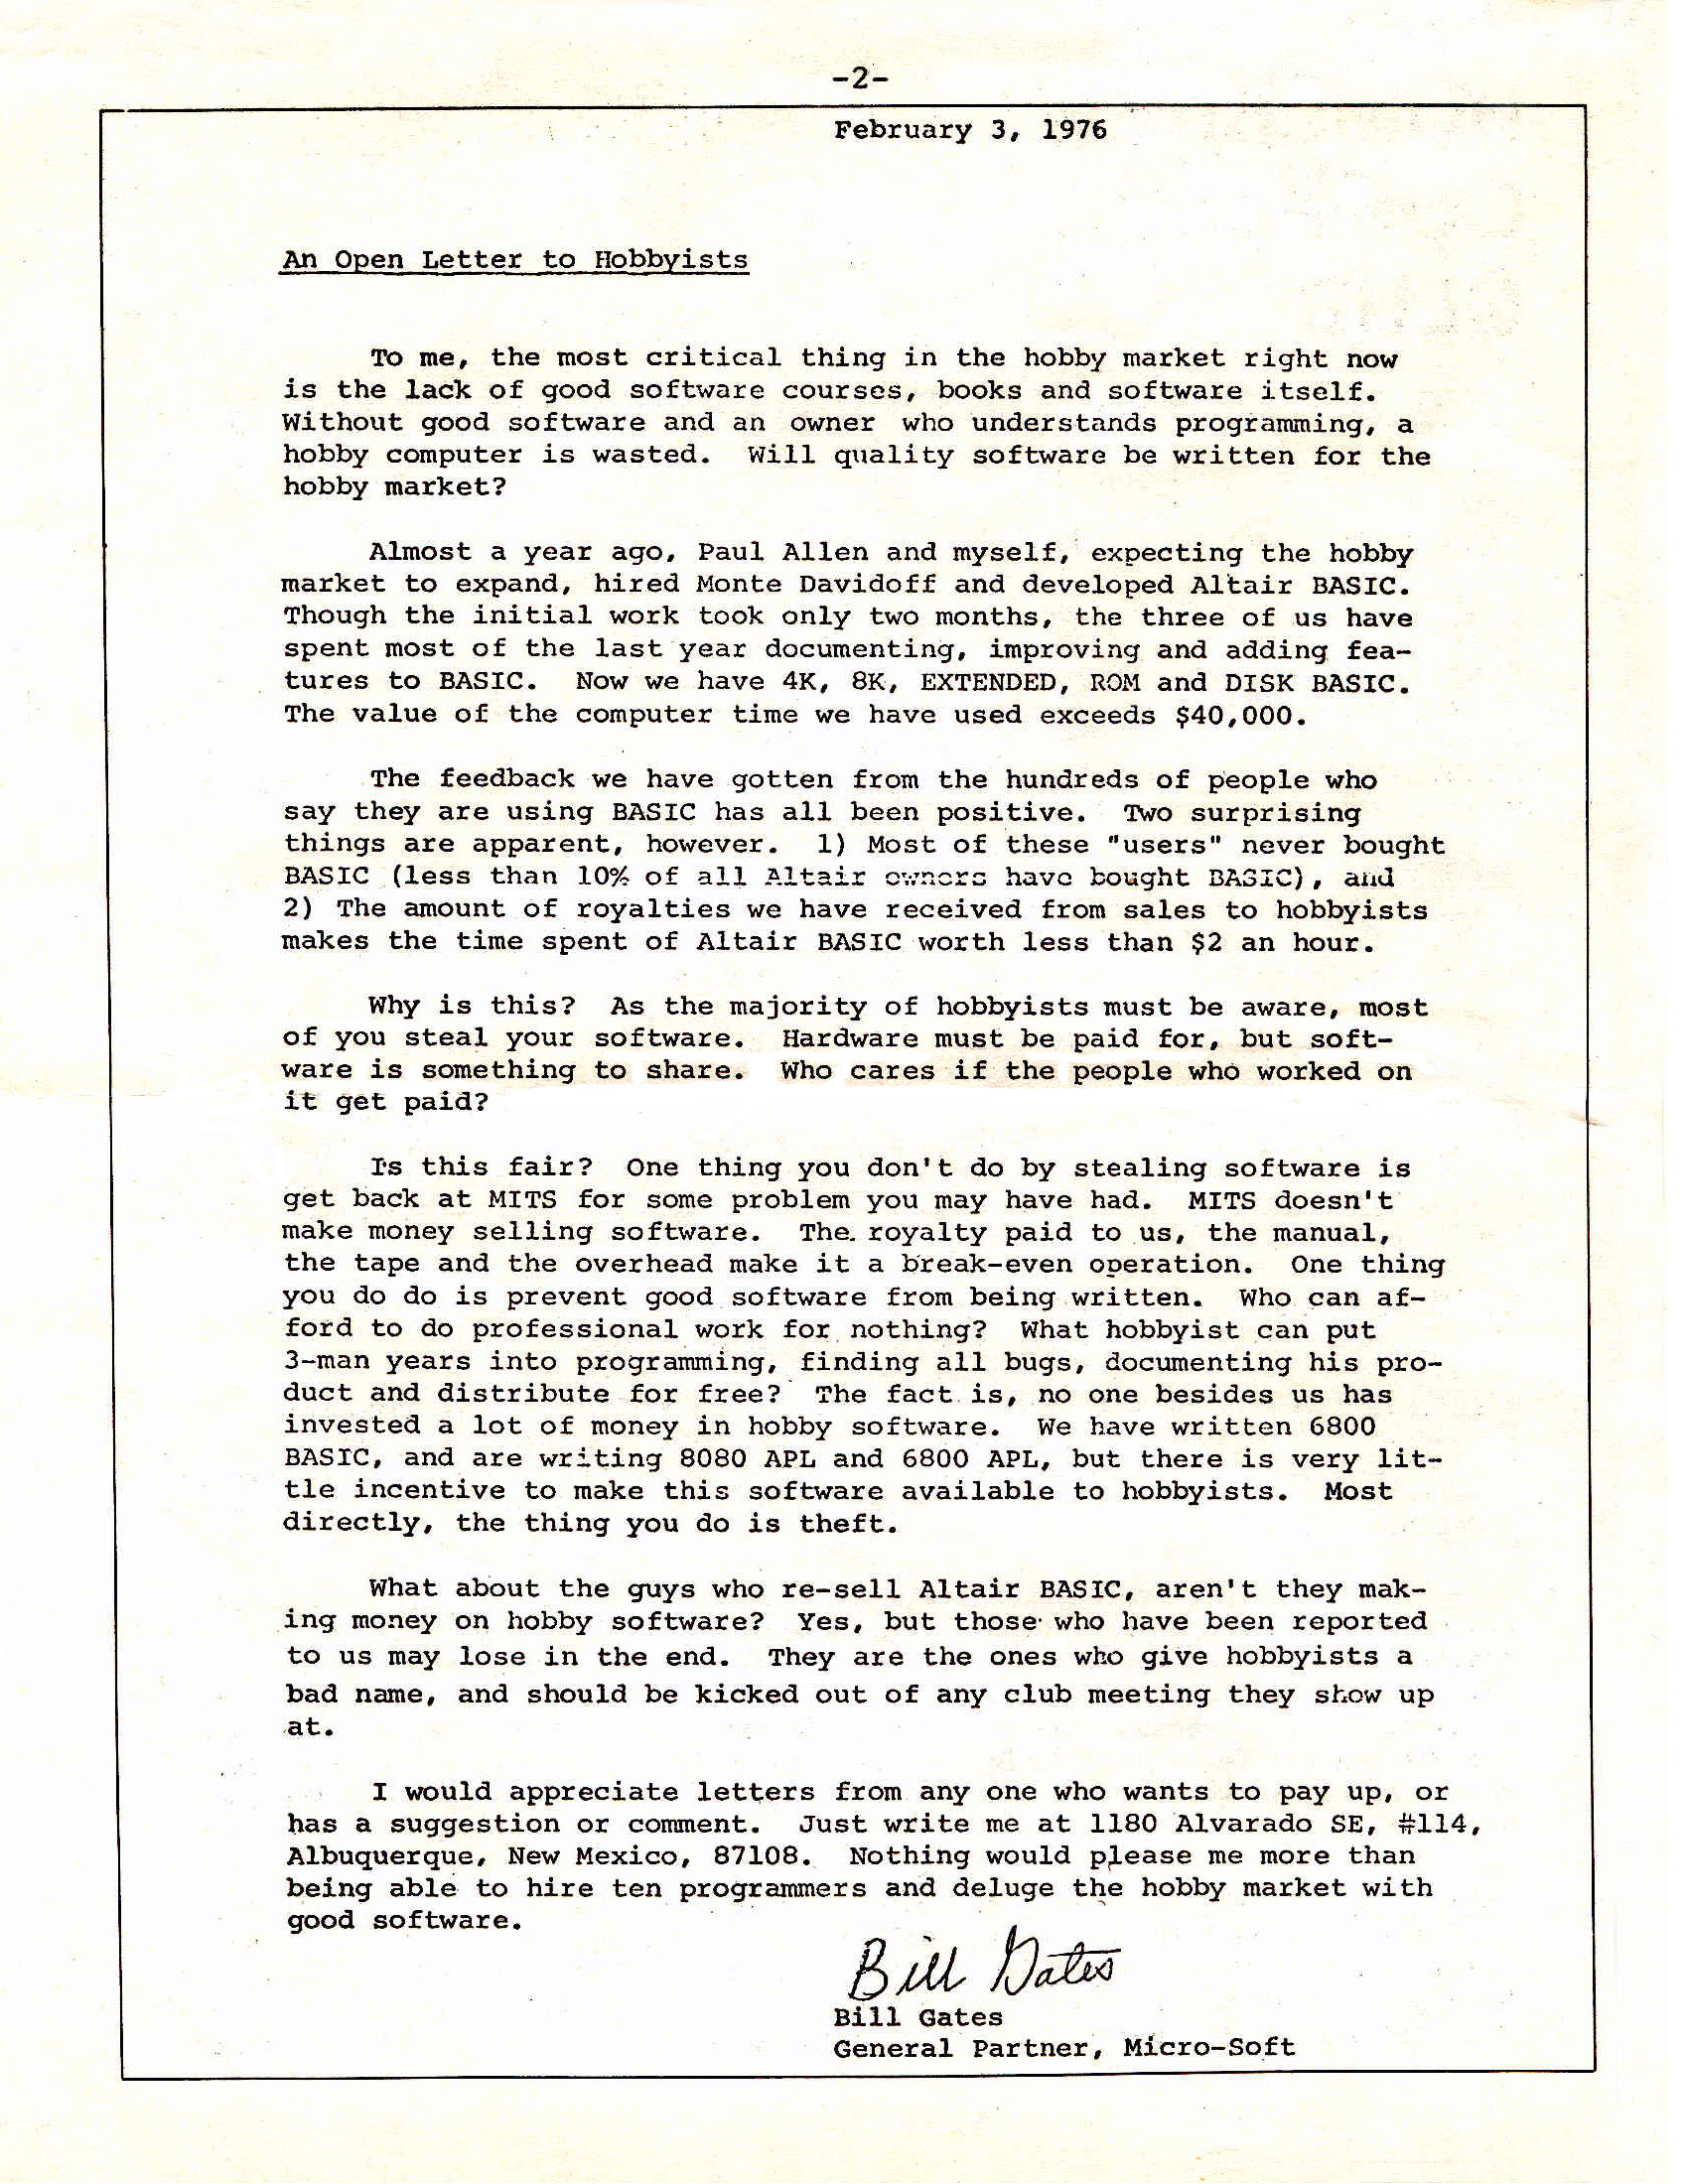
\includegraphics[width=5in]{Bill_Gates_Letter_to_Hobbyists.jpg}
\end{figure}

\subsection{1984}

During the rest of the decade, the mass marketing of the personal computer and new telecommunications technology like the acoustic coupler allowed phreaks and hackers to begin to communicate via computerized bulletin board systems. Hobbyists would have a computer hooked up to a perpetually open line which anyone could dial into. The users would upload and download files, messages, programs, etc. The culture was also transmitted via the local hacking and phone phreaking communities, where there would be meetups and people getting to know one another as people in meat-space.  The co-evolution of the network of bulletin board systems and the ARPANET built alongside and finally interconnected with the ARPANET that cause inter-cultural tension to this day. The ARPANET's development has been extensively documented by scholars such as Janet Abbate.
\footnote{Abbate, \emph{Inventing the Internet}} 
As the links between these hobby systems and the growing system of inter-networked computers became more complex it became what we think of as the Internet today. A distinct culture was built with the interaction of computers attached to the telephone network, being used, not for it’s popular purpose of voice communications, but instead being used to transmit computer data between hobbyists and a number of entrepreneurial computer operators.
\footnote{Jason Stott, \emph{BBS: The Documentary} 2005.}

By this point, computer bulletin boards had already started popping up all over the country. Hobbyists were connecting their computers to their phone lines and allowing others to dial in and leave messages, programs, and ascii based art. The Textfiles.com archive contains 58,227 files, adding up to over a billion bytes of information.
\footnote{Jason Stott, "Textfiles.com File Statistics," Jul 1 2005, http://www.textfiles.com/filestats.html.}
The focus of the archive is of this period before the Internet became accessible to people outside of major institutions. By 1984, there was already a major motion picture dramatizing the myth of the teenage hacker almost kick-starting the apocalypse, the Department of Justice had already produced a report on the techniques and standards required for computer security.
\footnote{Donn B. Parker, et al, \emph{Computer Crime: Computer Security Techniques} (US DOJ Bureau of Justice Statistics and SRI International, 1982).}
This document explicitly states the position that the information contained in computers is an asset, that computer security is necessary, and that opens up companies to liability if they don't perform due diligence in securing things like customer data and personal information, etc.

At this moment in 1984, the publication of a couple of renowned magazines begins to transmit the values and norms of hacker culture. \emph{Phrack Magazine} is an underground e-zine, ostensibly published out of The Metal Shop BBS. Craig Neidorf and Randy Tischler, known as Knight Lightning and Taran King, were the ones behind this.

The Table of Contents, below, illustrates the topics that are discussed by the popular hacker culture to this day.  From this, it's easy to see how hackers began to get linked inextricably with computer security, and security in general. Often, those who were outside of universities, corporations, or the military still wanted access to the computing resources. Some were espionage agents, some were just curious. Many hackers' first recourse was to just go ahead and access the systems without worrying overmuch about the legality. At that time, it was seen as a harmless exploration, akin to trespassing. This changed in 1986 with the passing of the Computer Fraud and Abuse Act, 18 U.S.C. § 1030. The penalties became much stricter after this. Violators were generally facing decades of jail-time with no opportunity for parole.

\begin{quote}
Volume One, Issue One, released on November 17, 1985. Included 
are: \\
1 This Introduction to Phrack Inc. by Taran King\\
2 SAM Security Article by Spitfire Hacker\\
3 Boot Tracing on Apple by Cheap Shades \\
4 The Fone Phreak's Revenge by Iron Soldier \\
5 MCI International Cards by Knight Lightning \\
6 How to Pick Master Locks by Gin Fizz and Ninja NYC \\
7 How to Make an Acetylene Bomb by The Clashmaster \\
8 School/College Computer Dial-Ups by Phantom Phreaker
\footnote{Knight Lightning, "Table of Contents" \emph{Phrack}, no 1. (March 1984)}
\\
\end{quote}

\emph{Phrack} does not mention anything about information freedom for quite some time. This is unexpected in one of the most famous hacker cultural artifacts. Instead, Knight Lightning responds to the phrase in a flippant manner. It seems that "information should be free" was a common truism. "Information shouldn't be free, you should find out things on your own."
\footnote{Knight Lightning, \emph{Phrack World News} XV, Part One -  July 27, 1986.}
The slogan was so accepted that it doesn't even need to be discussed directly, though Mr. Lightning seemed to have a different take on it.

\begin{quote}Knowledge is the key to the future and it is FREE. The telecommunications and
security industries can no longer withhold the right to learn, the right to
explore, or the right to have knowledge. The new age is here and with the use
of every *LEGAL* means available, the youth of today will be able to teach the
youth of tomorrow.\footnote{ibid. Issue XVIV/1. 1988.}\end{quote}

This citation from a couple years later was linked to the hacker ethic in that it advocated access for the purposes of education and exploration. Hackers even began noticing that their community was being discussed by academics, and went as far as to publish copies of the papers within the pages, 'lectronic\footnote{Yes, this is a reference to the WELL, Whole Earth 'Lectronic Link} or otherwise, of their publications.

\begin{quote}
Levy (1984) and Landreth (1985) both note that some computer aficionados have
developed a "hacker ethic" allowing harmless computer exploration, including
free access to files belonging to other users, bypassing passwords and security
systems, outwitting bureaucrats preventing access, and opposing private
software and copy protection schemes.
\footnote{Richard C. Hollinger, "Computer Hackers Follow A Guttman-Like Progression,"  \emph{Phrack Magazine} (2.22 File 7 of 12. 1988).}
\end{quote}

1984 also brings us the publication of the first issues of \emph{2600: The Hacker Quarterly} Including this powerful example of what it means to be a hacker.
\footnote{"The Constitution of a Hacker," \emph{2600 Magazine} (March 1984 V1 3).}
Edited by the pseudonymous Emmanuel Goldstein and published out of New York, this 'zine published exploits, code, news, and pictures of payphones from around the world.

\begin{figure}[ht!]
\center
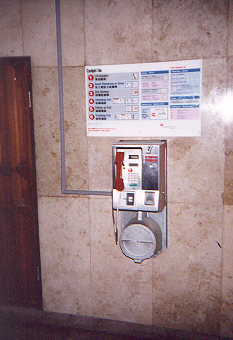
\includegraphics[width=60mm]{in003.jpg}
\caption{Payphone, Delhi, India \emph{2600 Magazine: The Hacker Quarterly} http://www.2600.com/phones/phonepics/in003.jpg}
\end{figure}

The Hacker Ethic, and the generation of a culture surrounding computers necessarily began within the institutional environments ultimately provided by DARPA. A conspiracy theorist might want to argue that it was an intentionally created thing, like an intentionally seeded counter-cultural inoculation that trained a legion of young people in the bread-and-butter of the (then) future of espionage and spy-craft. The ones who get punished aren't necessarily the technical wizards.
\footnote{Brian Knappenberger and John Dragonetti, \emph{We are legion the story of the hacktivists} (Venice, California: Luminant Media 2012) and Bruce Sterling, \emph{The Hacker Crackdown: Law and disorder on the digital frontier} (Bantam, 1992).} 
Often, those who crafted the programs and wrote the viruses passed them along via an anonymous BBS upload for others to implement and use.

The problem with taking the whole freedom of information thing too far leads us to diatribes from people like DIzzIE's "Why I Steal from Libraries."
\footnote{DIzzIE, "Why I Steal from Libraries" (Textfiles.com 2007) http://textfiles.com/uploads/diz-libraries.txt.} 
Apparently, the restrictions to have to check the books out or read them in the library are incompatible with information freedom. While it's easy to understand some of this person's concerns, the existence of this 2007 electronic tract illustrates how some people take the second tenet to give them the right to access any information that they seek without barrier and apparently without regard for others' ability to have that same access. This idea has since expanded to suggest not only the right but the moral duty to actively liberate information, so that it can be free for anyone to access.

The Internet is a system that was designed to survive the Apocalypse. Abstract away the loss of a city to a simple node going down, but the network, and therefore, the nation, civilization, humanity, survives. The laws that we have in place now were created during this time when the US was involved in a war of espionage and secrecy versus foreign powers. The people dialing into military or industrial systems seemed to be domestic enemies of the state. Some claimed the ability to subvert everything that held the social order together.
\footnote{\emph{Government Computer Security: Weak Computer Security in the Government: Is the Public at Risk with the U.S. Permanent Subcommittee on Investigations of the Senate Committee on Governmental Affairs} 105th Cong. (1998) statement of L0pht Heavy Industries.}
And even today, governments and corporations are routinely penetrated by unwanted intruders that the public believes are called hackers.

\newpage
\section{GNU, the GPL, and Linux}

\begin{figure}[ht!]
\center
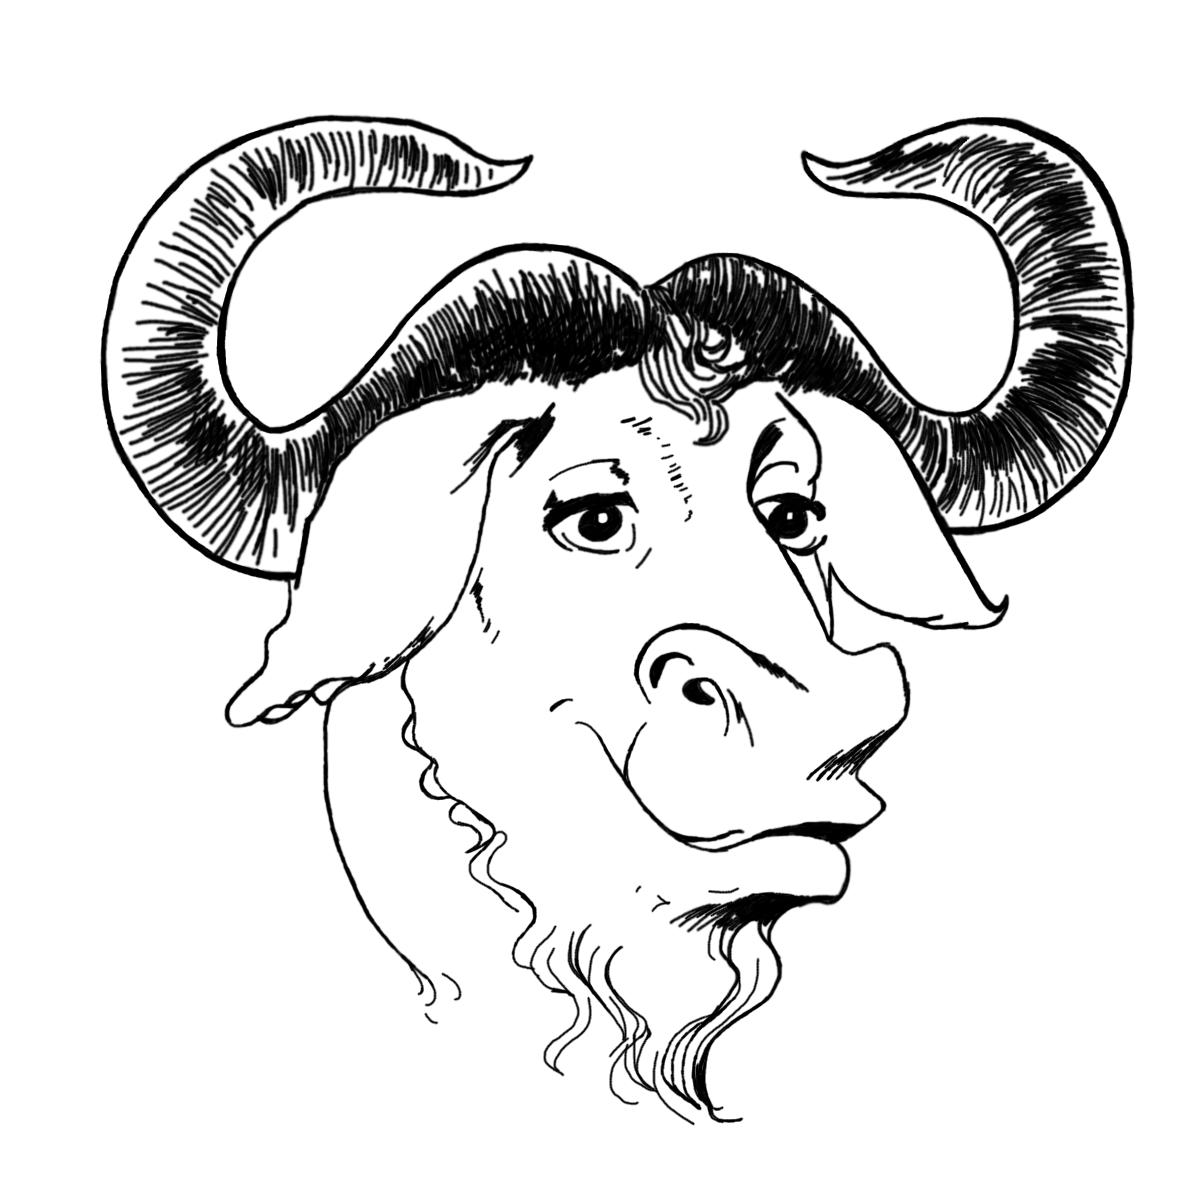
\includegraphics[width=100mm]{gerwinski-gnu-head.png}
\caption{A GNU Head by Etienne Suvasa http://www.gnu.org/graphics/agnuhead.html}
\end{figure}

\subsection{GNU ideas and the GPL}

During the 1980s, Richard Stallman announces the GNU project and begins constructing a free alternative for the UNIX operating system, which is not independently usable until the 1990s when GNU and Linux both fit together to form a fully functioning operating system. This was the genesis. The culmination of this was realized with the marriage, or at least bizairre mating experiment, of the Linux and GNU projects. The POSIX standards complient applications, GNU, and the POSIX standards complient kernel, Linux, happened to happily steamroll the competition to world domination The kernel is the name of a program that directs the scheduling and resource allocation to other programs. The POSIX standards are a common standard by which an operating system should be contacted to perform certain tasks like saving a file, or allocating resources to begin running a new program that the user has requested.

While most people with access to computing machines were playing games that they bought at their local retailer or happily using BBS systems. They were running whatever software they could get their hands on that would work on their machine. Sometimes there was a certain kind of elite hacker who even had access to the larger university systems and who had larger problems to boot, pun intended. The man in particular is known to hackers as "rms", but his government name is Richard Stallman. He has been the head of the free software movement and the Free Software Foundation since 1985. He is also known as the author of the GNU Public License, which has become the de-facto standard for licensing free software projects. He founded the GNU project, a collection of tools that comprise a free replacement for Unix.

His first conflict with proprietary software concerned the driver for a Xerox printer that the AI Lab at MIT was given in the early 70s. This particular printer had a penchant for jamming itself up, and as it was tucked away in another room, there was often a frustrating wait until someone actually realized the thing was jammed. Stallman had the idea to program the printer to notify users that there was a jam via a message to their terminal so that the printer would be able to be unjammed as needed. Xerox denied his requests for a copy of the source.

\begin{quote}
And then I heard that somebody at Carnegie Mellon University had a copy
of that software.  So I was visiting there later, so I went to his
office and I said, "Hi, I'm from MIT. Could I have a copy of the printer
source code?"  And he said "No, I promised not to give you a
copy." [Laughter]  I was stunned.  I was so -- I was angry, and I had no
idea how I could do justice to it.  All I could think of was to turn
around on my heel and walk out of his room.  Maybe I slammed the door.
[Laughter] And I thought about it later on, because I realized that I was
seeing not just an isolated jerk, but a social phenomenon that was
important and affected a lot of people.
\footnote{Richard Stallman, "Free Software: Freedom and Cooperation" (Speech Transcript. NYU, 29 May 2001) http://www.gnu.org/events/rms-nyu-2001-transcript.txt.}
\end{quote}

After this incident, he began a crusade to create a world in which these problems would never happen again. The General Public License and GNU project aimed to create a legal framework and a collection of software published underneath this framework. It's known as copyleft, the opposite of copyright. Instead of controlling the work published under such a license, you are giving up those rights, but in an interesting twist of legalese, the license also carries a requirement for anyone who borrows your code to share any modifications, hopefully improvements, with the community as a whole.

\subsection{Minix, Linux, and an accidental avalanche}

In the late 80s, Andrew Tanenbaum created Minix as a simplified educational replacement for the UNIX operating system. This allowed students, such as then graduate student, Linus Torvalds, to learn how to put together the essential components of an operating system. He did, and then decided to release his operating system kernel under the GNU General Public License.

\begin{quote}
ALERT! WARNING! NOTE! These sources still need minix-386 to be compiled
  (and gcc-1.40, possibly 1.37.1, haven't tested), and you need minix to
  set it up if you want to run it, so it is not yet a standalone system
  for those of you without minix. I'm working on it. You also need to be
  something of a hacker to set it up (?), so for those hoping for an
  alternative to minix-386, please ignore me. It is currently meant for
  hackers interested in operating systems and 386's with access to minix.
  \footnote{Linus Torvalds, Usenet Posting in comp.os.minix 5 Oct 1991. http://www.cs.cmu.edu/~awb/linux.history.html Accessed 18 Feb 2013.}\end{quote}

With the development of the TCP protocol and continued expansion of the physical medium that gave more people the ability to obtain access, many hackers were able to get it, compile it, and run it.
\footnote{Nick McKeown and Phillip Levis, "Congestion Control - TCP Tahoe" (on-line lecture, Stanford, Fall 2012).} 
Now, with this kernel, and the rest of the components of the GNU free operating system, any hacker could have a UNIX-like operating system environment on the common Intel 386 platform. It took a few years for this to get really rolling, but today the majority of the servers connected to the Internet are running the Linux kernel, as well as most of the major supercomputing facilities, not to mention the millions of personal computers, a drop in the bucket, but a substantial drop.
\footnote{Linus Torvalds, Richard Stallman, Bruce Perens, Eric S. Raymond, Larry M. Augustin, Brian Behlendorf, Michael Tiemann, Susan Egan, and J. T. S. Moore. \emph{Revolution OS: hackers, programmers \& rebels unite.} (S.l.: Wonderview Productions, 2003).}
After years of being forced into disparate environments by proprietary fragmentation, home users had access to a system that was functionally similar to those being used to do advanced programming, graphics, and chip design tasks. Prior to this system, the programming environments that were available to home users did not have anything in common with the UNIX systems that were doing the heavy lifting in industry.

\newpage

\section{Conclusion}

While the world was dealing with the criminal expression of the hacker ideals through Operation Sundevil, the hackers themselves were organizing and programming their replacements to make the criminal expression obsolete. With the GNU/Linux system openly available to anyone, a person or another entity has the freedom to tailor a system exactly to their needs. This is the essential issue of free software and this marks one of the most important, if subtly acting, cultural events of the Computer Revolution.

Hackers gave us the ability to create a virtual public sphere and with the Arab Spring, hacktivist movements, open culture movements, and the networks of Occupy protests, many have put these spheres to active use.
\footnote{J\"urgen Habermas, "The Public Sphere: An Encyclopedia Article" \emph{New German Critique} (No 3. Autumn, 1974) 49-55.}
It's possible here to suggest that we are creating the foundations  of a post nationalist global society within cyberspace.
\footnote{J\"urgen Habermas, \emph{The Postnational Constellation} (Cambridge, Mass ; London: MIT Press 2001).} These international links are the actually powerful thing that has come out of the wiring of the planet. While anthropomorphizing technology is a problematic stance to take. We can't ignore Kevin Kelley, proprietor of Wired magazine.
\footnote{Kevin Kelley, \emph{What Technology Wants}, (Viking 2010).} It's no joke that this is the first time in the history of this planet that someone programming a computer in Taiwan can have an almost instantaneous impact on computer systems, thereby people, in Texas. Moving bits around theoretically is inconsequential, but the messages in those bits can expose corruption, organize citizens to action, even topple governments. We all need active users such as hackers, who are exploring the limits and edges of the system, to balance against the powerful interests that claim ownership and control of the networks. Hackers have historically driven innovation in unexpected ways. 

Hackers are a popular counter-cultural movement that has had an impact on the way almost everyone interacts with the world around them. It follows that the culture has successfully evolved in an increasingly hostile world.
\footnote{Margaret Mead, \emph{Continuities in Cultural Evolution}. (New Haven: Yale University Press, 1964).}
Hackers are credited, or blamed, as the first people that leveraged the potential for interactive computing. Because of the hackers' desire to wrangle directly with the computer, the nature of work has changed for many people all over the world. This subculture has since bloomed in a new cultural niche.

The problem with this bloom is that the core values held by this culture have clashed with normal cultural values time and time again. Information has never been free in a cultural environment of war, secret weapons, military intelligence, trade secrets and intellectual property. When the majority of people with political clout see ideas as a capital investment, it's difficult to legitimize an ideal that these ideas should be freely distributed. If industrialists had their way, we'd be ignorantly buying at the monopolistic company store. Sadly, this is how the vast majority of people tend to interact with computing technology as a whole. Vast computer industrial empires have been created based on the general ignorance of the public. This is a bad thing. The largest stash of US dollars in the world was amassed by charging "for what could be dirt cheap if it wasn't run by profiteering gluttons."
\footnote{The Mentor "The Hacker Manifesto" (Jan 8, 1986) http://www.mithral.com/~beberg/manifesto.html.}
And because the industry is so entrenched and much the public is so vehement about keeping their workflow exactly the same, a totally free alternative has a minimal market share on desktop systems. This is contrasted it's in use by the vast majority of supercomputing and server systems. The numbers are almost juxtaposed, with 90 percent Windows usage on desktop systems, versus about 1 percent. Actually, there are only 3 of the top 500 supercomputers using a Windows-based system, so the disparity is even more extreme than that.
\footnote{Net Market Share, "Market Share Statistics for Internet Technologies" http://www.netmarketshare.com/ and "Top 500 Supercomputer Sites" http://www.top500.org}
The people who are making the decisions about important scientific computing are making different choices. Maybe it's time for the rest of the world to catch up and realize that a used computer with a free GNU/Linux based system can perform every mission critical task aside from those that are.

\newpage
\section{Appendix}

\begin{singlespace}
\noindent I like to think (and\\
the sooner the better!)\\
of a cybernetic meadow\\
where mammals and computers\\
live together in mutually\\
programming harmony\\
like pure water\\
touching clear sky.\\

\noindent I like to think\\
\indent (right now, please!)\\
of a cybernetic forest\\
filled with pines and electronics\\
where deer stroll peacefully\\
past computers\\
as if they were flowers\\
with spinning blossoms. \\

\noindent I like to think\\
\indent (it has to be!)\\
of a cybernetic ecology\\
where we are free of our labors\\
and joined back to nature,\\
returned to our mammal\\
brothers and sisters,\\
and all watched over\\
by machines of loving grace.
\footnote{Brautigan, Richard. "All Watched Over by Machines of Loving Grace". San Francisco. The Communication Company. 1967. Print.}
\end{singlespace}
\newpage



\newpage
\section{Bibliography}
\begin{hangparas}{15pt}{1}
Abbate, Janet. \emph{Inventing the Internet} Cambridge: MIT Press, 1999.

Brautigan, Richard. "All Watched Over by Machines of Loving Grace," San Francisco: The Communication Company, 1967.

Breen, C. and Dahlbom, C. A. "Signaling Systems for Control of Telephone Switching," \emph{The Bell System Technical Journal} 39:6. Nov 1960.

Chaos Computer Congress. "Hackerethik," Berlin 2013. http://ccc.de/de/hackerethik.

Coleman, Gabriela. \emph{Coding Freedom.} Princeton: Princeton University Press, 2013.

Digital Equipment Corporation \emph{Digital Equipment Corporation: Nineteen Fifty-Seven to the Present,} DEC Press (1978): http://www.computerhistory.org/collections/accession/102630349.

DIzzIE, "Why I Steal from Libraries" Textfiles.com, (2007): http://textfiles.com/uploads/diz-libraries.txt.

\emph{Government Computer Security: Weak Computer Security in the Government: Is the Public at Risk with the U.S. Permanent Subcommittee on Investigations of the Senate Committee on Governmental Affairs}, 105th Cong. (1998) statement of L0pht Heavy Industries

Gates, Bill. "An Open Letter to Hobbyists" \emph{Various Sources} (1975) http://en.wikipedia.org/wiki/Open\_Letter\_to\_Hobbyists.

Habermas, Jurgen. \emph{The Postnational Constellation}, Cambridge, Mass ; London : MIT Press 2001.

Habermas, Jurgen, "The Public Sphere: An Encyclopedia Article" \emph{New German Critique} (No 3. Autumn, 1974) 

Headrick, Daniel. \emph{The Invisible Weapon} (New York: Oxford University Press, 1991)

Headrick, Daniel. \emph{When Information Came of Age.} (New York : Oxford University Press. 2000).

Himanen, Pekka. \emph{The Hacker Ethic, and the Spirit of the Information Age}. (New York: Random House. 2001.)

Hollinger, Richard C. "Computer Hackers Follow A Guttman-Like Progression"  \emph{Phrack Magazine} (2.22 File 7 of 12. 1988)

Holt, Thomas J. "Subcultural Evolution? Examining the Influence of On and Off-line Experiences on Deviant Subcultures. \emph{Deviant Behavior} 28:2

IHTFP FAQ,  http://hacks.mit.edu/Hacks/misc/faq.html, accessed Feb 2013

Johns, Adrian. \emph{Piracy: The Intellectual Property Wars from Gutenberg to Gates}. Chicago: University of Chicago Press, 2010.

Kelley, Kevin, \emph{What Technology Wants}. Viking, 2010.

Kelty, Chris. \emph{Two Bits : The Cultural Significance of Free Software}. Durham: Duke University Press, 2008.

Kline, Katy, "A Brief Architectural History of MIT" \emph{Art and Architecture at MIT: A Walking Tour of the Campus}. Cambridge: MIT Press, 1988.

Knappenberger, Brian, and John Dragonetti. \emph{We are legion the story of the hacktivists.} Venice, California: Luminant Media, 2012.

Knight Lightning. \emph{Phrack World News.} Issue XV: Part One -  July 27, 1986

Knight Lightning, "Table of Contents" \emph{Phrack}, no 1. (March 1984)

Lubar, Stephen. ""Do Not Fold, Spindle or Mutilate": A Cultural History of the Punch Card," \emph{Journal of American Culture} 15, no. 4 (1992) 43-55.

McKeown, Nick and Phillip Levis, "Congestion Control - TCP Tahoe" On-line Lecture, Stanford 2012.

Mead, Margaret. \emph{Continuities in Cultural Evolution}, New Haven: Yale University Press, 1964.

Net Market Share, "Market Share Statistics for Internet Technologies" http://www.netmarketshare.com/ 

"Top 500 Supercomputer Sites" http://www.top500.org

Parker, Donn B, \emph{Fighting Computer Crime,} New York: Scribner, 1983.

Parker, Donn B. et al, \emph{Computer Crime: Computer Security Techniques} US DOJ Bureau of Justice Statistics and SRI International, 1982.

Raymond, Eric S. \emph{The Jargon File version 4.4.7} 2003.  http://www.catb.org/jargon/html/H/hacker.html.

Raymond, Eric S. \emph{The New Hacker's Dictionary - 3rd edition}, Cambridge: The MIT Press, 1996.

Raymond, Eric S. "How To Become A Hacker," 20 May 2012. http://www.catb.org/esr/faqs/hacker-howto.html.

Rosenbaum, Ron, "Secrets of the Little Blue Box" \emph{Esquire} 1971.

Schroeder, Steve. \emph{The Lure the True Story of How the Department of Justice Brought Down Two of the World's Most Dangerous Cyber Criminals}, Boston: Course Technology PTR, 2012. http://site.ebrary.com/id/10448180.

Spinrad, Paul and Patti Meagher. "Project Genie: Berkeley’s piece of the computer revolution." \emph{Forefront}, Fall 2007, http://coe.berkeley.edu/news-center/publications/forefront/archive/forefront-fall-2007/features/berkeley2019s-piece-of-the-computer-revolution.

Stallman, Richard. "Free Software: Freedom and Cooperation." Speech Transcript. NYU. 29 May 2001, http://www.gnu.org/events/rms-nyu-2001-transcript.txt.

Stallman, Richard. "On Hacking." 2002, http://stallman.org/articles/on-hacking.html.

Stallman, Richard. "On Hacking." 2002, http://stallman.org/articles/on-hacking.html.

Sterling, Bruce. \emph{The Hacker Crackdown: Law and disorder on the digital frontier.} Bantam, 1992.

Stott, Jason. \emph{BBS: The Documentary} 2005.

Stott, Jason. "Textfiles.com File Statistics," Jul 1 2005, http://www.textfiles.com/filestats.html.

"The Constitution of a Hacker." \emph{2600 Magazine.} (March 1984 V1 3)

The Mentor "The Hacker Manifesto" Jan 8, 1986 http://www.mithral.com/~beberg/manifesto.html

Thomas, Douglas. \emph{Hacker Culture} Minneapolis: University of Minnesota, 2002.

Torvalds, Linus, Richard Stallman, Bruce Perens, Eric S. Raymond, Larry M. Augustin, Brian Behlendorf, Michael Tiemann, Susan Egan, and J. T. S. Moore. \emph{Revolution OS: hackers, programmers \& rebels unite.} S.l.: Wonderview Productions, 2003.

Torvalds, Linus. "Usenet Posting in comp.os.minix," 5 Oct 1991. Accessed 18 Feb 2013. http://www.cs.cmu.edu/~awb/linux.history.html.

United States Congress. "The Effects of Nuclear War." by Lionel S. Johns, et al., Washington, D.C.:GPO, 1979, http://ota.fas.org/reports/7906.pdf.

Wark, McKenzie. \emph{A Hacker Manifesto.} Cambridge, MA : Harvard University Press, 2004.

Weizenbaum, Joseph. "Science and the compulsive programmer." \emph{Computer Power and Human Reason.} San Fransisco: W.H. Freeman and Company, 1976.
\end{hangparas}
\end{document}